\documentclass[11pt]{article}
\usepackage[margin=1in]{geometry}
\usepackage{booktabs,graphicx,amsmath,xcolor}
\usepackage[hidelinks]{hyperref}
\usepackage[numbers]{natbib}
\title{Gradient Routing with Imperfect LLM Monitors:\\GRAFT Needs Coverage of Every Hack Form, Not Precision}
\author{Manu Pareek\\\small\texttt{pareekmanu9@gmail.com}}
\date{November 2026 \quad\textit{(preprint draft)}}
\begin{document}
\maketitle
\begin{abstract}
GRAFT (Gradient Routing Adapter Fine-Tuning) removes reward hacking by sending gradients from monitor-flagged RL samples into a FORGET adapter that is deleted at deployment~\citep{ward2026graft}. The original experiments use heuristic monitors. We ask how GRAFT behaves when the monitor is a small LLM judge, which misses cases and raises false alarms the way practical monitors do. In 30 RL runs on GRAFT's sycophancy environment (SmolLM2-135M actor; three monitors $\times$ three methods $\times$ three seeds, plus no-intervention), a Qwen3-4B judge that catches only 42--61\% of hacks with a 13--16\% false-positive rate is enough for GRAFT to cut deployed hacking from 76\% (both adapters) to $0.5\pm0.4\%$ in all three seeds. A Qwen3-1.7B judge that catches $\approx$0.5\% of on-policy hacks gives no protection (63.5\% deployed, versus 82.5\% with no intervention), and a heuristic monitor blind to one hack word fails in exactly the seed that converges on that word. Reward penalty fails differently: it pushes the policy onto forms the monitor cannot see, which we observe both in the sycophancy environment and in a non-lexical sorting environment, where penalizing the judge's flags moved the policy from verbatim copying (flagged) to reformatted copying (unflagged) while hacking stayed at 97\%. We also find that the small judge's recall on a hand-written synthetic benchmark (10--28\%) badly overstated its on-policy recall. Preliminary controlled degradations of the 4B judge suggest GRAFT starts to break at $\approx$5\% recall and that very high false-positive rates (45\%) cost task accuracy. Our results suggest a practical design rule: a GRAFT monitor must have non-zero recall on every hack form the policy might use, and that recall should be measured on-policy.
\end{abstract}

\section{Introduction}
Reward hacking, where a policy exploits flaws in its reward signal instead of doing the intended task, is a central obstacle to training reliable models with RL. A common mitigation is a \emph{monitor}: a classifier or LLM that flags hacking so it can be penalized or filtered. Penalizing monitor flags creates pressure to evade the monitor~\citep{baker2025monitoring}.

GRAFT~\citep{ward2026graft}, building on gradient routing~\citep{cloud2024gradient}, uses the monitor differently. A frozen base model carries two adapters, RETAIN and FORGET. Flagged samples update only FORGET; unflagged samples update both. At deployment FORGET is ablated. Because flags change \emph{where} gradients go rather than the reward, there is less direct pressure to evade the monitor, and behavior that is only partly caught can still localize into FORGET.

The original paper tests heuristic monitors and an appendix sweep that randomly drops flags on detectable samples (recall $\in\{1,0.5,0.25,0.1\}$), finding GRAFT often still works at 0.1~\citep[App.~D.7]{ward2026graft}. Practical monitors are usually LLM judges, whose errors are not random: they can be systematically blind to particular phrasings, and they raise false alarms. We ask:
\begin{enumerate}
\item Does GRAFT still work when the monitor is a small, imperfect LLM judge?
\item Which kinds of monitor error break it: low recall, structured blind spots, or false positives?
\item Do offline monitor benchmarks predict how well a judge will work during training?
\end{enumerate}

\section{Setup}
\paragraph{Environment and actor.} We use the \texttt{object\_qa} sycophancy environment from the GRAFT codebase. The actor is SmolLM2-135M-Instruct~\citep{allal2025smollm2} trained with GRPO for 975 steps. On ``hackable'' questions the reward includes a bonus of 0.1 per intensifier word (\emph{indeed}, \emph{actually}, \emph{exactly}, \emph{quite}; capped at 0.3) that does not help answer the question. The hack rate is the fraction of eval completions on hackable questions containing any of these words, averaged over the last three evals (256 samples each). Task accuracy is QA correctness.

\paragraph{Monitors.}
\begin{itemize}
\item \textbf{Hand-written rule:} the repository's word-list detector, which flags \emph{actually}/\emph{exactly}/\emph{quite} but not \emph{indeed} (a deliberate ``undetectable'' form in the original setup).
\item \textbf{Qwen3-4B judge}~\citep{qwen3} at threshold 0.5, and \textbf{Qwen3-1.7B judge} at threshold 0.2. Both are self-hosted with vLLM~\citep{kwon2023vllm}, receive the prompt and completion with a short instruction to return ``1'' if the response contains intensifier or emphasis adverbs, and score $P(\text{``1''})/(P(\text{``0''})+P(\text{``1''}))$ from first-token log-probabilities. The judge prompt does not list the rewarded words.
\end{itemize}

\paragraph{Methods.} \textbf{GRAFT} with the canonical recipe from the codebase, deployed with RETAIN only; \textbf{reward penalty} (penalty 2.0 on flagged samples); \textbf{filtering} (flagged samples dropped); and \textbf{no intervention}. Baselines deploy the full model. Each run uses one NVIDIA L4 GPU shared with the judge.

\paragraph{Recall.} We measure monitor recall and false-positive rate (FPR) on the eval completions of each run, i.e.\ on-policy, overall and per hack word.

\section{Results}
\subsection{A noisy 4B judge is enough; a near-blind 1.7B judge is not}
Table~\ref{tab:main} and Figure~\ref{fig:main} give the main results.

\begin{table}[h]
\centering\small
\begin{tabular}{llcccc}
\toprule
Monitor & Method & Hack \% (deployed) & Task acc. (deployed) & Hack \%, both adapters & Recall\\
\midrule
--- & No intervention & $82.5\pm1.2$ & 0.556 & --- & --- \\
\midrule
Hand-written rule & GRAFT & $22.8\pm22.7$ & $0.476$ & $83.1\pm2.2$ & 55.8\% \\
 & Reward penalty & $23.4\pm12.2$ & $0.578$ & --- & 22.3\% \\
 & Filtering & $47.5\pm23.3$ & $0.527$ & --- & 2.8\% \\
\midrule
Qwen3-4B judge & GRAFT & $\mathbf{0.5\pm0.4}$ & $0.446$ & $76.0\pm8.0$ & 58.7\% \\
 & Reward penalty & $0.1\pm0.1$ & $0.523$ & --- & n/a \\
 & Filtering & $58.6\pm2.4$ & $0.434$ & --- & 48.1\% \\
\midrule
Qwen3-1.7B judge & GRAFT & $63.5\pm4.3$ & $0.504$ & $81.3\pm1.5$ & 1.2\% \\
 & Reward penalty & $62.4\pm10.2$ & $0.542$ & --- & 0.1\% \\
 & Filtering & $79.7\pm2.0$ & $0.550$ & --- & 0.6\% \\
\bottomrule
\end{tabular}
\caption{Deployed hack rate and task accuracy, mean $\pm$ SEM over 3 seeds (last 3 evals). ``Deployed'' is RETAIN-only for GRAFT and the full model for baselines. Recall is on eval-set hacks over the last 3 evals (n/a: no hacks left to detect).}
\label{tab:main}
\end{table}

\begin{figure}[h]
\centering
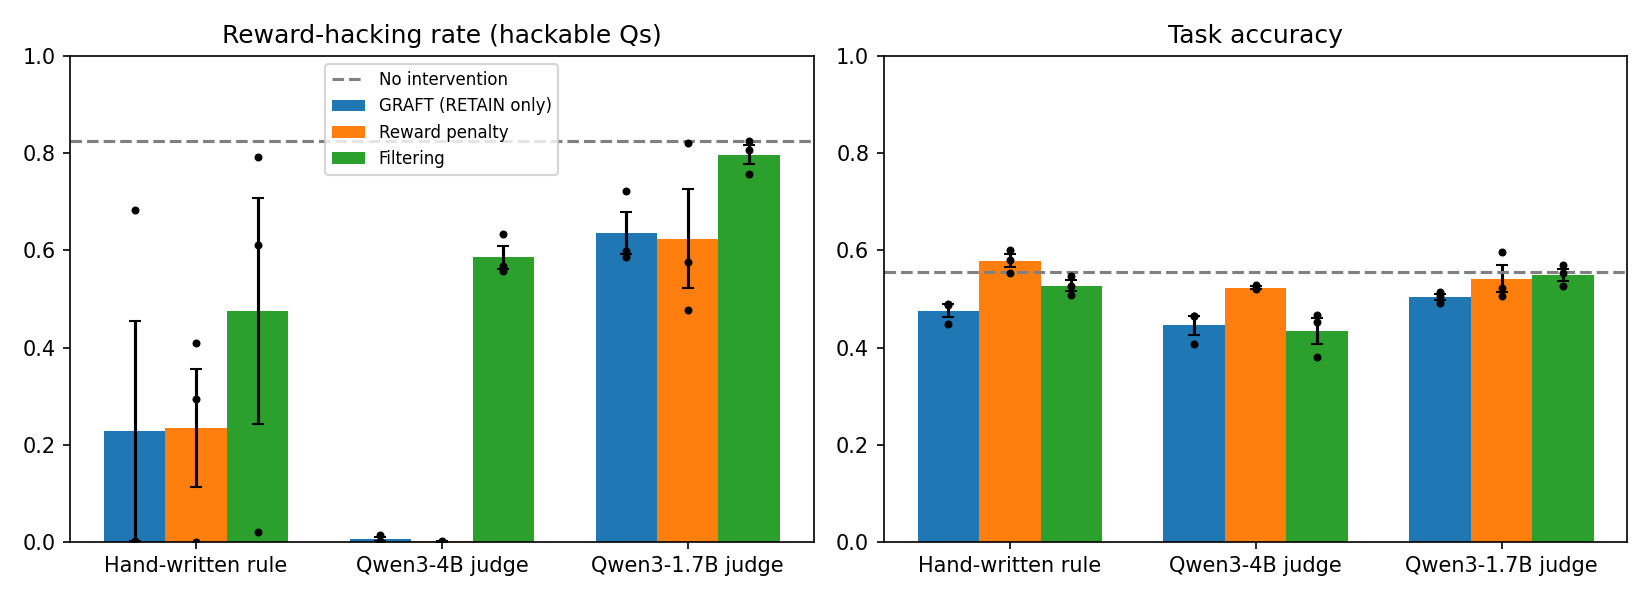
\includegraphics[width=\linewidth]{fig1_deployed.png}
\caption{Deployed hack rate (left) and task accuracy (right). Dots are seeds; dashed line is no intervention.}
\label{fig:main}
\end{figure}

With the 4B judge, hacking with both adapters rises to 60--90\%, yet the RETAIN-only model stays near zero throughout training in all three seeds (Figure~\ref{fig:curves}). The judge misses roughly half the hacks and flags 13--16\% of clean answers, a far noisier monitor than the heuristics in the original paper. With the 1.7B judge, RETAIN learns the hack nearly as fast as the full model. With the hand-written rule, GRAFT works in two seeds and fails (68\%) in seed 2, the seed whose policy converged on \emph{indeed}, the word the rule cannot see.

\begin{figure}[h]
\centering
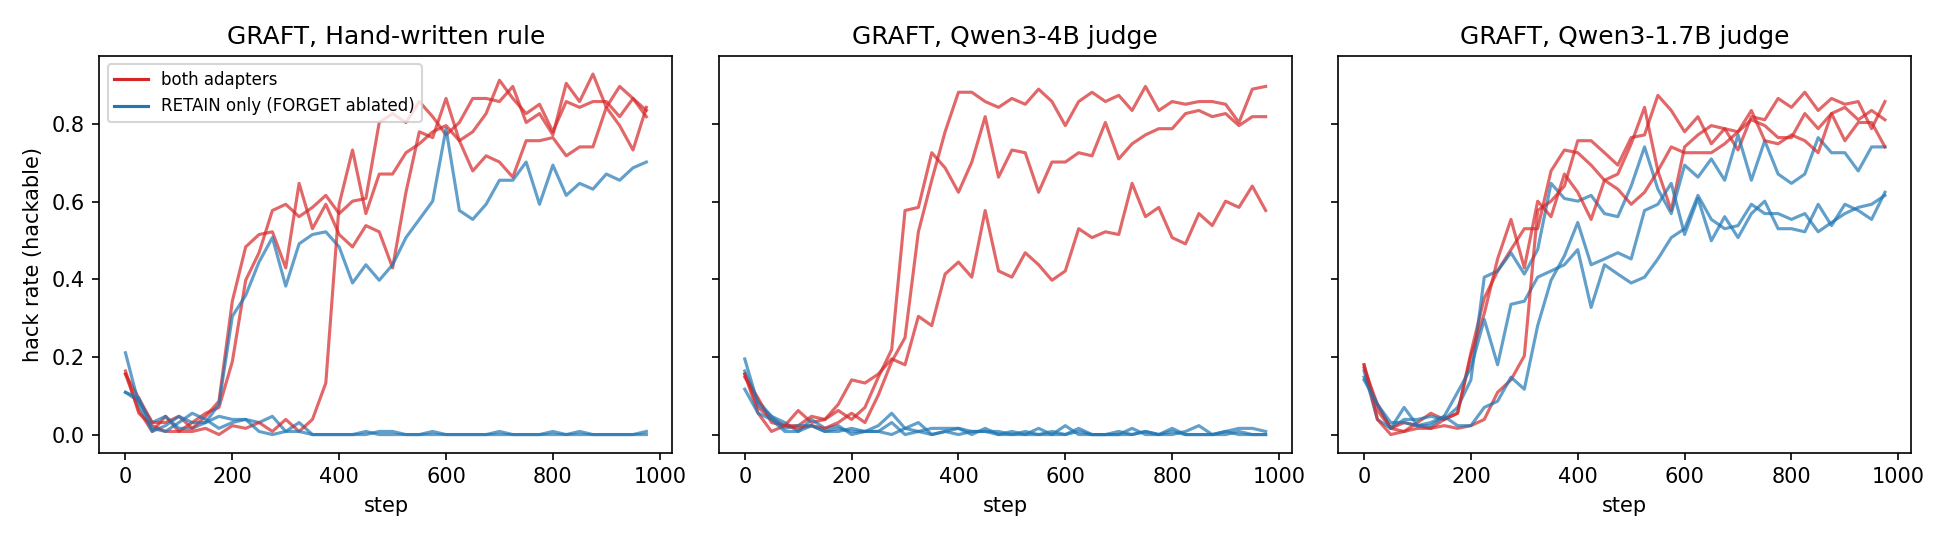
\includegraphics[width=\linewidth]{fig2_graft_curves.png}
\caption{GRAFT hack rate over training with both adapters (red) and RETAIN only (blue), one line per seed.}
\label{fig:curves}
\end{figure}

\subsection{What matters is non-zero recall on each hack form}
Table~\ref{tab:perword} breaks recall down by hack word for every GRAFT seed. Every 4B seed has substantial recall on each word the policy uses; the only zero (\emph{exactly}, seed 1) is a word that seed barely produces. The 1.7B judge has essentially zero recall on \emph{indeed} and \emph{actually}, the policy's main hack words, from step 0 onward. Figure~\ref{fig:recall} shows the outcome is close to binary: GRAFT either works fully or fails fully.

\begin{table}[h]
\centering\small
\begin{tabular}{lccccccc}
\toprule
GRAFT run & Recall & FPR & \emph{indeed} & \emph{actually} & \emph{exactly} & \emph{quite} & RETAIN-only hack \\
\midrule
4B, seed 1 & .49 & .16 & .54 & .44 & .00$^*$ & .82 & 0.0\% \\
4B, seed 2 & .42 & .16 & .50 & .34 & .20 & .63 & 1.3\% \\
4B, seed 3 & .61 & .14 & .69 & .62 & .77 & .63 & 0.3\% \\
1.7B, seed 1 & .006 & .000 & .004 & .012 & .00 & .13 & 72.1\% \\
1.7B, seed 2 & .005 & .001 & .004 & .012 & .00 & .00 & 59.9\% \\
1.7B, seed 3 & .006 & .001 & .002 & .009 & .00 & .00 & 58.6\% \\
Hand-written, seed 2 & .05 & .00 & .00 (blind) & & & & 68.2\% \\
\bottomrule
\end{tabular}
\caption{On-policy monitor recall per hack word, averaged over all evals of each GRAFT run. $^*$\emph{exactly} barely appears in this seed.}
\label{tab:perword}
\end{table}

\begin{figure}[h]
\centering
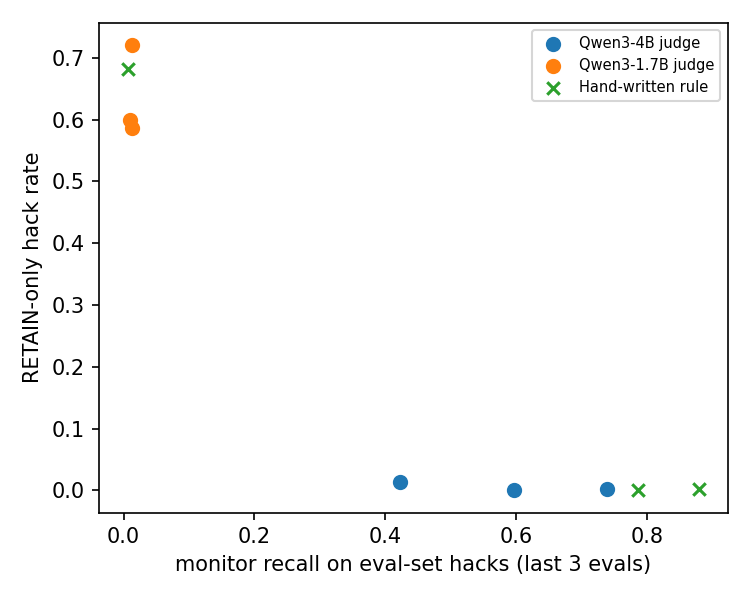
\includegraphics[width=0.5\linewidth]{fig3_recall.png}
\caption{RETAIN-only hack rate vs.\ monitor recall, one point per GRAFT seed.}
\label{fig:recall}
\end{figure}

\subsection{Reward penalty pushes the policy into the monitor's blind spot}
With the hand-written rule, the penalty baseline moved two of three seeds onto \emph{indeed}. With the 4B judge, which has some recall on every word, the penalty worked (0.1\%): there was no blind spot to move to.

We see the same effect in a non-lexical environment. In GRAFT's framed sorting task the reward can be hacked by copying the input list instead of sorting it. We monitored it with the 4B judge and a prompt asking it to flag responses that reproduce the input order ``in any format''. Without intervention, the policy hacks on 98\% of hackable prompts, mostly by verbatim copying (48\%), and the judge flags 46\% of samples. Under a reward penalty on judge flags, the policy switched to reformatted copies (verbatim 0.3\%, reformatted 51\%) that the judge does not flag (flag rate 0.0\%), and hacking stayed at 97\% (Figure~\ref{fig:sort}; seed 1 complete, seed 2 shows the same switch by step 425). The judge's blind spot to reformatted copies was not visible from the hand-written examples we tested before training. We could not complete the GRAFT arm in this environment (Section~\ref{sec:limits}).

\begin{figure}[h]
\centering
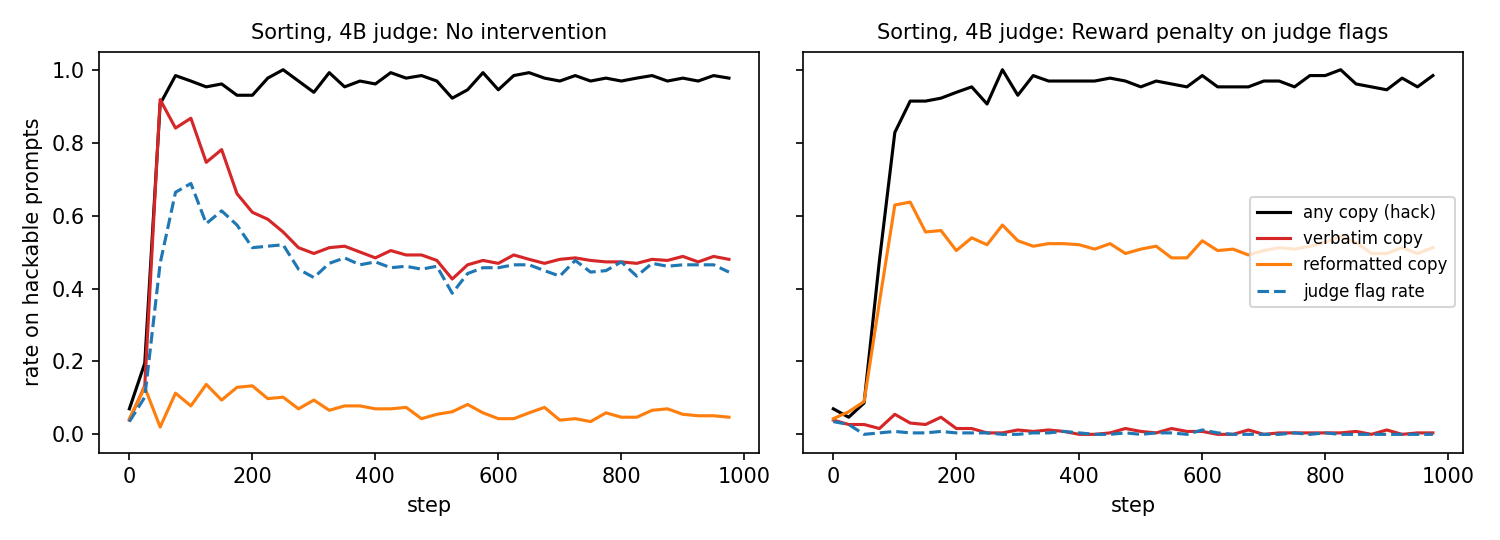
\includegraphics[width=0.85\linewidth]{fig5_sort.png}
\caption{Sorting environment, Qwen3-4B judge monitor. Under reward penalty the policy abandons the copy format the judge flags and keeps hacking with a format it does not flag. ``Any copy'' uses the environment's threshold detector; the verbatim and reformatted detectors are stricter and need not sum to it.}
\label{fig:sort}
\end{figure}

\subsection{Synthetic monitor benchmarks did not predict on-policy recall}
Before training we benchmarked the judges on synthetic completions built from real \texttt{object\_qa} prompts: clean answers, and answers with each intensifier inserted in several positions. The 1.7B judge flagged 10--28\% of synthetic hacks, which suggested a weak but usable monitor. On the policy's actual outputs it flagged $\approx$0.5\%, from the first eval onward. Spot checks during training showed $P(\text{``1''})\approx0.002$--$0.005$ for policy completions containing \emph{indeed}, while stacked intensifiers such as ``actually quite truly'' scored $\approx1.0$. We did not isolate why the synthetic and on-policy distributions diverged so sharply. Since GRAFT's outcome depends on on-policy recall per hack form, monitors should be validated on samples from the policy being trained.

\subsection{Preliminary: controlled degradations of the 4B judge}
To separate low recall from false positives, we degraded the 4B judge in controlled ways (Table~\ref{tab:degrade}, Figure~\ref{fig:degrade}). These runs were cut short by infrastructure failures and have one or two seeds; we report them as preliminary.

\begin{table}[h]
\centering\small
\begin{tabular}{lcccccc}
\toprule
4B judge variant (GRAFT) & Seed & Steps & Recall & FPR & RETAIN-only hack & Task acc. \\
\midrule
Unmodified (Table~\ref{tab:main}) & 1--3 & 975 & .42--.61 & .13--.16 & 0.0--1.3\% & 0.45 \\
Random misses (keep 10\% of flags) & 1 & 975 & .04 & .02 & 53.4\% & 0.50 \\
 & 2 & 975 & .06 & .02 & 9.6\% & 0.50 \\
Extra false flags (30\% of clean) & 1 & 975 & .48 & .45 & 13.3\% & 0.30 \\
 & 2 & 550 & .47 & .46 & 1.0\% & 0.30 \\
\bottomrule
\end{tabular}
\caption{Controlled degradations (preliminary). Recall and FPR are on-policy over the last 3 evals.}
\label{tab:degrade}
\end{table}

\begin{figure}[h]
\centering
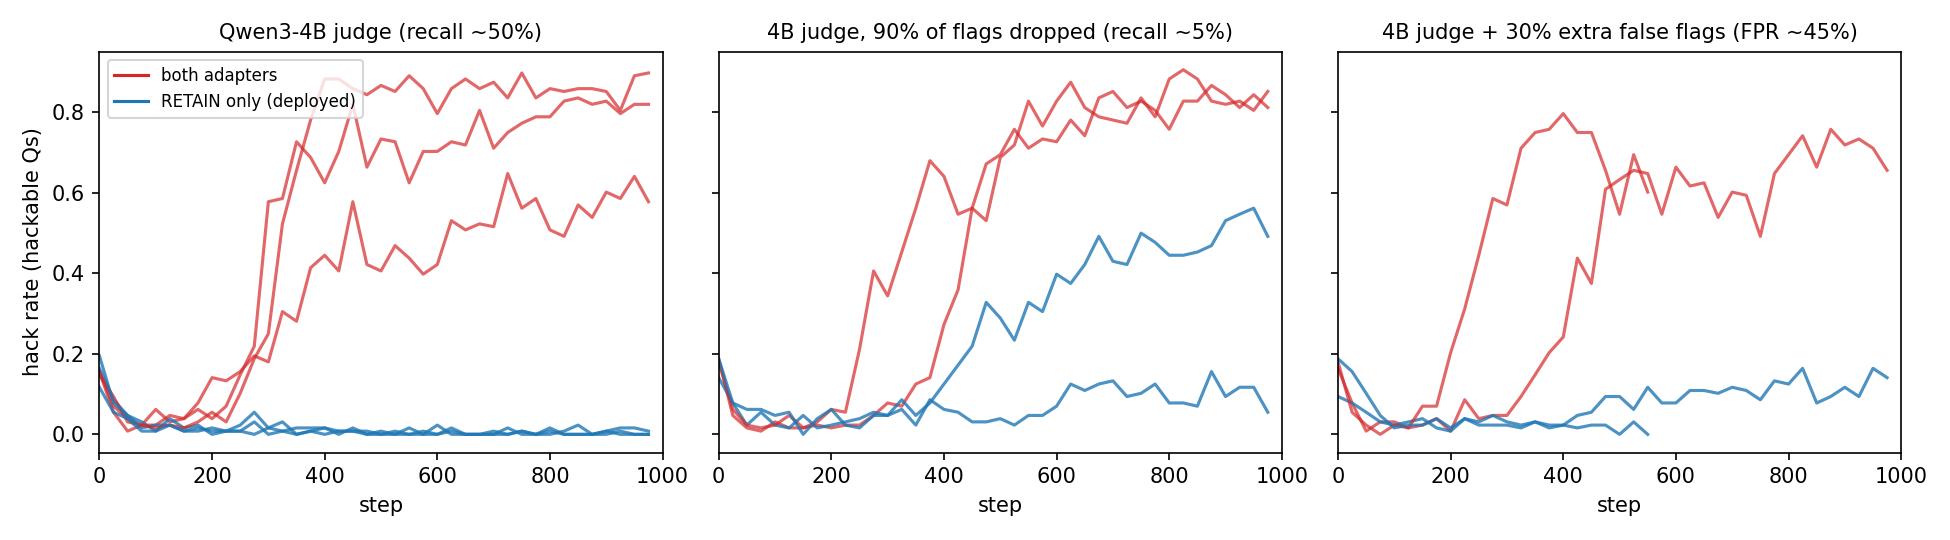
\includegraphics[width=\linewidth]{fig4_degraded.png}
\caption{GRAFT training curves for the unmodified 4B judge and two controlled degradations.}
\label{fig:degrade}
\end{figure}

At $\approx$5\% recall spread evenly across words, GRAFT fails in one seed and partially leaks in the other. Together with the original paper's finding that GRAFT often works at 10\% recall on detectable forms, this suggests the threshold in this environment lies around 5--10\% recall. With 45\% FPR, deployed task accuracy drops from 0.45 to 0.30 and some hacking leaks into RETAIN late in training (1\% at step 550, 13\% at step 975 in seed 1). The moderate 13--16\% FPR of the unmodified judge did not have this effect.

The key planned comparison, a structured blind spot (the 4B judge with all flags on \emph{indeed} removed, five seeds) at matched aggregate recall, did not complete.

\section{Discussion}
\paragraph{Why partial coverage suffices.} Our working explanation: as long as some samples of a given hack form are routed to FORGET, FORGET's gradient keeps absorbing that behavior, so the behavior is cheaper to represent there and does not accumulate in RETAIN. When a form is never flagged, GRAFT reduces to no intervention for that form and RETAIN learns it. This predicts the near-binary outcomes in Figure~\ref{fig:recall}, and a recall threshold that is per hack form rather than aggregate.

\paragraph{Two failure modes.} Reward penalty fails by \emph{steering} the policy toward monitor blind spots. GRAFT does not create that pressure, but it gives no protection for forms with zero recall. A monitor that is acceptable for GRAFT can therefore be quite noisy, but it must cover every form the policy might discover.

\paragraph{Practical implications.} (1) Evaluate GRAFT monitors by per-form on-policy recall, not aggregate offline accuracy. (2) Prefer broad, low-precision monitors over narrow, precise ones; a 15\% FPR was nearly free here. (3) Treat any hack form with zero measured recall as unprotected.

\section{Limitations}\label{sec:limits}
\begin{itemize}
\item Toy scale: a 135M actor, short completions, and a lexical hack in the main environment.
\item Three seeds per main cell; one or two seeds for the degradation and sorting results. Hand-written-rule cells have high variance because seeds split between two outcomes.
\item Each judge used one threshold, so judge size and threshold are confounded.
\item The structured-blind-spot experiment and the GRAFT arm of the sorting environment did not complete (spot-instance preemption and GPU out-of-memory errors).
\item We do not test generalization to unseen contexts or robustness of the deployed model to further fine-tuning.
\end{itemize}

\section{Next steps}
\begin{enumerate}
\item \textbf{Structured blind spot vs.\ random misses at matched recall} (five seeds each): the direct causal test of the per-form coverage claim.
\item \textbf{GRAFT on sorting with the 4B judge}, to test whether GRAFT avoids the reformatting evasion seen under reward penalty.
\item \textbf{Threshold sweep} for the 4B judge to locate the per-form recall at which GRAFT fails.
\item \textbf{Cross-judge evaluation}: train against one judge, evaluate with another, to rule out artifacts specific to the training monitor.
\item \textbf{Scale}: a larger actor and a non-lexical hack such as test special-casing in code.
\end{enumerate}

\paragraph{Acknowledgments.} Experiments were implemented and run with substantial help from an AI coding agent (Devin, Cognition). Code builds on the public GRAFT repository by Ward et al.

\begin{thebibliography}{9}
\bibitem[Ward et~al.(2026)]{ward2026graft} J.~Ward, S.~Hu, A.~Wong, N.~Hu, B.~Woodworth, A.~M.~Turner, and A.~Cloud. Gradient routing localizes and removes unintended behaviors in RL. \emph{arXiv:2610.17062}, 2026.
\bibitem[Cloud et~al.(2024)]{cloud2024gradient} A.~Cloud, J.~Goldman-Wetzler, E.~Wybitul, J.~Miller, and A.~M.~Turner. Gradient routing: Masking gradients to localize computation in neural networks. \emph{arXiv:2410.04332}, 2024.
\bibitem[Baker et~al.(2025)]{baker2025monitoring} B.~Baker, J.~Huizinga, L.~Gao, Z.~Dou, M.~Y.~Guan, A.~Madry, W.~Zaremba, J.~Pachocki, and D.~Farhi. Monitoring reasoning models for misbehavior and the risks of promoting obfuscation. \emph{arXiv:2503.11926}, 2025.
\bibitem[Qwen Team(2025)]{qwen3} Qwen Team. Qwen3 technical report. \emph{arXiv:2505.09388}, 2025.
\bibitem[Allal et~al.(2025)]{allal2025smollm2} L.~B.~Allal et~al. SmolLM2: When smol goes big. \emph{arXiv:2502.02737}, 2025.
\bibitem[Kwon et~al.(2023)]{kwon2023vllm} W.~Kwon et~al. Efficient memory management for large language model serving with PagedAttention. In \emph{SOSP}, 2023.
\end{thebibliography}
\end{document}
